\chapter{The Neoclassical Growth Model}

The fundamental departure of the Neoclassical Growth Model from the Solow model is that \textbf{growth through capital accumulation is driven by an endogenous saving rate ($s$)}. We no longer assume a mechanical rule; instead, we build the economy from the ground up using microeconomic optimization.

\section{The Economic Environment}

We consider an infinite-horizon discrete-time economy where time is indexed by $t = 0, 1, 2, \dots$. The economy consists of two types of rational agents interacting in perfectly competitive markets.
\begin{itemize}
    \item \textbf{A Representative Household (HH):}
    \begin{itemize}
        \item Endowed with an initial capital stock $K_0$ and a constant labor supply $L$.
        \item At each period $t$, the HH provides capital $K_t$ and labor $L$ to the market, earning a wage $w_t$ and a capital rental rate $r_t$.
        \item The HH must decide how much to consume and how much to invest/save ($I_t$) for the future.
    \end{itemize}
    \item \textbf{A Representative Firm:}
    \begin{itemize}
        \item At each period $t$, the firm buys (rents) capital $K_t$ and labor $L_t$ from the HHs.
        \item The firm pays the factor prices $r_t$ and $w_t$ to produce output.
        \item The production function is given by $AF(K_t, L_t)$, where $F$ exhibits constant returns to scale (CRS) and has positive marginal products ($F_K > 0, F_L > 0$), and $A$ represents the total factor productivity (TFP).
    \end{itemize}
    \item \textbf{Market Structure}\\
    All markets are perfectly competitive, meaning households and firms are strict price-takers (i.e., they have zero market power and treat all prices as exogenous constants in their optimization problems). The sequence of market prices is given by:
\begin{itemize}
    \item Final good price: $P_t$\footnote{A ``final good" refers to a product that is in its end-use stage (i.e., used directly for either household consumption $C_t$ or capital investment $I_t$), as opposed to intermediate goods which are used up during the production process.}
    \item Labor wage: $w_t$
    \item Capital rental rate: $r_t$
\end{itemize}
\end{itemize}

\rmkb[``Representative" and ``Aggregation'']{
The term ``representative" implicitly assumes there is a continuum of identical households and firms, both normalized to a total measure of 1. The key of the macroeconomic aggregation is \textit{not} that the number of firms equals the number of households. Instead, it is the fundamental asymmetry between technology and preferences. Because the firm's technology is Constant Returns to Scale (scale-free), the number of firms is mathematically irrelevant. However, because the household's utility function is strictly concave (scale-dependent), we \textit{must} normalize the continuum of households to a measure of 1. This normalization allows us to safely study a single representative individual's intertemporal choice without loss of generality.
}

\section{The Household's Problem}

The representative household is forward-looking and maximizes its infinite-horizon discounted lifetime utility, taking the sequence of prices $\{P_t, r_t, w_t\}_{t=0}^\infty$ as given.

The HH's sequence problem is formulated as:\footnote{Technically, the household derives utility from its individual consumption $c_t$. However, because we assume a representative household normalized to a measure of 1, individual consumption equals aggregate consumption ($c_t = C_t$). Standard macro notation uses capital letters directly in the utility function to reflect this equivalence.}
$$
\max_{\{C_t, K_{t+1}\}_{t=0}^\infty} \sum_{t=0}^\infty \beta^t u(C_t)
$$
subject to the dynamic period-by-period budget constraint. Conceptually, the household's total nominal expenditure on consumption ($C_t$) and investment ($I_t$) must equal its total nominal income:
$$
P_t (C_t + I_t) = w_t L + r_t K_t + \Pi_t
$$
Recall the fundamental law of motion for capital: tomorrow's capital is today's un-depreciated capital plus today's investment, $K_{t+1} = (1-\delta)K_t + I_t$. Substituting the implied investment $I_t = K_{t+1} - (1-\delta)K_t$ into the equation yields the standard formulation:
$$
\underbrace{P_t \left[ C_t + K_{t+1} - (1-\delta)K_t \right]}_{\text{Expenditure}} = \underbrace{w_t L + r_t K_t + \Pi_t}_{\text{Income}}, \quad \forall t \ge 0
$$
with initial conditions and non-negativity constraints: $K_0, L$ given, and $C_t \ge 0$ for all $t$.

In the HH's problem,
\begin{itemize}
    \item $\beta \in (0,1)$ is the time discount factor, capturing the HH's patience.
    \item $u(C_t)$ is the period utility function. The standard assumptions are $u' > 0$ (more is better) and $u'' < 0$ (diminishing marginal utility). The strict concavity of the utility function ($u'' < 0$) mathematically drives the desire for \textit{endogenous consumption smoothing}.
    \item $\Pi_t$ represents the profit remitted from the firms to the households (who are the ultimate owners of the firms).
\end{itemize}

\section{The Firm's Problem}

Unlike the household, which faces a dynamic intertemporal problem, the representative firm solves a sequence of \textit{static} optimization problems. Capital is rented period-by-period, so the firm faces no dynamic state variables.

Taking the sequence of prices $\{P_t, w_t, r_t\}_{t=0}^\infty$ as given, the firm chooses input demands $\{K_t, L_t\}$ at each period $t$ to maximize profit:
$$
\Pi_t = \max_{\{K_t, L_t\}} P_t A F(K_t, L_t) - r_t K_t - w_t L_t。
$$

\section{Competitive General Equilibrium}

Having specified the micro-foundations—the household's dynamic optimization and the firm's static optimization—we can now define the macroeconomic equilibrium. This definition perfectly mirrors the standard Walrasian General Equilibrium from microeconomic theory.

\defn{Competitive General Equilibrium}{

A \textit{competitive general equilibrium} is defined as a sequence of prices $\{P_t, r_t, w_t\}_{t=0}^\infty$ and a sequence of allocations $\{C_t, L_t, K_{t+1}\}_{t=0}^\infty$ such that:
\begin{enumerate}
    \item \textbf{Household Optimization:} Given the price sequence $\{P_t, r_t, w_t\}_{t=0}^\infty$, the allocation $\{C_t, K_{t+1}\}_{t=0}^\infty$ solves the representative household's utility maximization problem.
    \item \textbf{Firm Optimization:} Given the price sequence $\{P_t, r_t, w_t\}_{t=0}^\infty$, the allocation $\{K_t, L_t\}_{t=0}^\infty$ solves the representative firm's profit maximization problem period by period.
    \item \textbf{Markets Clear:} All markets in the economy must clear simultaneously at every period $t$:
    \begin{itemize}
        \item \textbf{Goods Market Clearing:} The total supply of goods $F(K_t, L)$ equals the total demand for goods (consumption plus investment):
        $$
        C_t + \underbrace{K_{t+1} - (1-\delta)K_t}_{I_t} = AF(K_t, L) \quad \forall t
        $$
        \item \textbf{Labor Market Clearing:} Firm's labor demand equals household's labor supply:
        $$
        L_t = L \quad \forall t
        $$
    \end{itemize}
\end{enumerate}
}

\rmkb[]{
    The Neoclassical Growth Model is fundamentally a \textit{real economy} model. There is no fiat money, no central bank, and no financial nominal frictions. Transactions are essentially barters (i.e., direct exchanges of goods and services without the use of money) of real goods for real factors of production.

Mathematically, if the sequences $\{P_t, w_t, r_t, C_t, L_t, K_{t+1}\}_{t=0}^\infty$ constitute a general equilibrium, then for any arbitrary sequence of strictly positive scalars $\{\alpha_t\}_{t=0}^\infty > 0$, the scaled sequence:
$$
\{\alpha_t P_t, \alpha_t r_t, \alpha_t w_t, C_t, L_t, K_{t+1}\}_{t=0}^\infty
$$
is \textit{also} an equilibrium. 

This is a direct consequence of Walrasian demand and supply functions being \textit{homogeneous of degree zero} in prices. If both your income (wages and capital rents) and the price of consumption goods multiply by $\alpha_t$, your budget constraint remains perfectly unchanged. Therefore, your optimal real allocations ($C_t, K_{t+1}$) do not change. Only \textit{relative prices} (the real wage $w_t/P_t$ and the real rental rate $r_t/P_t$) matter for resource allocation. This is the precise mathematical reason why many advanced macroeconomics textbooks entirely omit the price level $P_t$ from the household's and firm's problems from the very beginning. They simply assume $P_t = 1$ for mathematical convenience, focusing exclusively on the relative real prices that actually dictate economic behavior.

As argued before, arbitrary sequence $\{\alpha_t\}$ has absolutely zero effect on real allocations ($C_t, K_{t+1}$). This demonstrates the \textit{classical dichotomy}: in a frictionless real model, nominal variables (inflation) are completely divorced from real variables (growth and consumption). While the classical dichotomy holds elegantly in this frictionless theoretical model, it generally fails in the real world. In reality, the macroeconomy is rife with \textit{nominal frictions} (e.g., sticky prices, long-term wage contracts). If prices and wages cannot adjust instantaneously and perfectly to scale with $\alpha_t$, then inflation will distort relative prices, erode real purchasing power, and have profound, tangible impacts on real economic variables.
}

To solve for the general equilibrium analytically, we extract the FOCs from both the household's and the firm's optimization problems and combine them.

Let $\lambda_t$ be the Lagrange multiplier associated with the HH's budget constraint at time $t$:
$$
\mathcal{L} = \sum_{t=0}^\infty \beta^t \left\{ u(C_t) + \lambda_t \left[ w_t L + (r_t + 1 - \delta)K_t + \Pi_t - C_t - K_{t+1} \right] \right\}
$$
Taking derivatives with respect to the choice variables $C_t$ and $K_{t+1}$ yields:
$$
\begin{aligned}
    \frac{\partial \mathcal{L}}{\partial C_t} = 0 \quad &\implies \quad u'(C_t) = \lambda_t \\
    \frac{\partial \mathcal{L}}{\partial K_{t+1}} = 0 \quad &\implies \quad \lambda_t = \beta \lambda_{t+1} (r_{t+1} + 1 - \delta)
\end{aligned}
$$
Combining these two first-order conditions, we obtain the Household's Euler equation:
$$
u'(C_t) = \beta u'(C_{t+1}) (r_{t+1} + 1 - \delta)
$$
\rmkb[Intuition of the HH's Euler Equation]{
    This is the fundamental intertemporal no-arbitrage condition. At the optimum, the household must be indifferent between consuming the marginal unit today versus investing it for tomorrow.
\begin{itemize}
    \item \textbf{LHS ($u'(C_t)$):} The marginal loss of saving. It is the utility you give up today by saving one extra unit of goods.
    \item \textbf{RHS ($\beta u'(C_{t+1}) (r_{t+1} + 1 - \delta)$):} The marginal gain from saving, evaluated at time $t$. If you save one unit today, it becomes capital tomorrow, survives depreciation ($1-\delta$), and earns the rental rate ($r_{t+1}$). This total return is then converted into tomorrow's marginal utility $u'(C_{t+1})$ and discounted back to today by $\beta$.
\end{itemize}
}

The representative firm solves a static profit maximization problem. Taking derivatives of $\Pi_t = P_t F(K_t, L_t) - r_t K_t - w_t L_t$ with respect to $L_t$ and $K_t$ yields:
$$
\begin{aligned}
    w_t &= P_tA F_L(K_t, L) \\
    r_t &= P_tA F_K(K_t, L) 
\end{aligned} 
$$
Because this is a real economy where only relative prices matter, the absolute price level is purely a scalar. For analytical simplicity, it is a universal convention in computation to normalize the price of the final good to unity ($P_t = 1 \quad \forall t$). Thus, the nominal factor prices perfectly equal their real marginal products: $w_t = F_L$ and $r_t = F_K$. 

We substitute the firm's real equilibrium rental rate $r_{t+1} = F_K(K_{t+1}, L)$ into the Household's Euler equation:
$$
u'(C_t) = \beta u'(C_{t+1}) \left[ AF_K(K_{t+1}, L) + 1 - \delta \right] \quad \cdots \text{(EE)}
$$

The beauty of the Neoclassical Growth Model is its \textit{block recursive} structure.\footnote{Mathematically, a system of equations is block recursive if it can be partitioned into blocks that can be solved sequentially. In our model, the equations determining real quantities ($C_t, K_t$) do not contain the price variables ($w_t, r_t$) once we substitute out the rental rate. Thus, we can solve for the real allocations first, and then recursively use those allocations to determine the implied prices.} We can decouple the real allocations from the prices. We can decouple the real allocations from the prices.

\prop{Equilibrium Characterization}{
Assuming Inada conditions hold\footnote{
    Inada conditions guarantee interior solutions $C_t > 0, K_t > 0$.
}, a sequence of prices and allocations $\{P_t, w_t, r_t, C_t, L_t, K_{t+1}\}_{t=0}^\infty$ is a general equilibrium {if and only if} it satisfies the Transversality Condition (TVC) 
\[
\lim_{t \to \infty} \beta^t u'(C_t) K_{t+1} = 0,
\] along with the following two sequential blocks:
\begin{itemize}
    \item \textbf{Block 1: Solving for Allocations (The Real Economy)} \\
    We completely ignore prices and solve a system of two difference equations for the two variables $\{C_t, K_{t+1}\}$:
$$
\begin{cases}
    \text{Euler Equation:} & u'(C_t) = \beta u'(C_{t+1}) \left[ AF_K(K_{t+1}, L) + 1 - \delta \right] \\
    \text{Market Clearing:} & C_t + K_{t+1} - (1-\delta)K_t = AF(K_t, L)
\end{cases}
$$
    \item \textbf{Block 2: Backing out Prices} \\
    Once the sequence of allocations $\{C_t, K_{t+1}\}$ is found, we simply plug them into the firm's FOCs to back out the equilibrium prices $w_t = AF_L(K_t, L)$ and $r_t = AF_K(K_t, L)$ period by period.
\end{itemize}
}

\rmkb[Why is the TVC Mathematically Necessary for a GE?]{
    In an infinite-horizon problem, the EE only prevents short-term (one-period) deviations. The TVC ($\lim_{t \to \infty} \beta^t u'(C_t) K_{t+1} = 0$) is required to prevent the household from over-accumulating capital forever without consuming it. But a natural question arises: how does ``over-accumulating capital forever'' break the definition of a general equilibrium? The answer lies strictly in the household optimization condition in the GE definition.
    
The Euler equation is only a \textit{local} first-order condition. It merely guarantees that the household cannot improve its lifetime utility by shifting consumption between any adjacent periods $t$ and $t+1$. However, in an infinite-horizon setting, local optimality does not guarantee global optimality.

Suppose a proposed equilibrium path satisfies the Euler equation and market clearing, but violates the TVC, meaning $\lim_{t \to \infty} \beta^t u'(C_t) K_{t+1} > 0$. This implies that the \textit{present utility value} of the capital stock left over at the ``end of time" is strictly positive. If this is true, the household is acting sub-optimally. The household could easily construct a strictly better feasible path: simply consume a tiny bit more at $t=0$ (which strictly increases lifetime utility) and let the entire future sequence of capital $\{K_t\}$ drift down by a small margin. Because the asymptotic present value of capital was strictly positive, this slight perpetual reduction will never cause $K_t$ to violate the non-negativity constraint ($K_t \ge 0$) even at infinity. 

Because a strictly better feasible consumption path exists, the original path \textit{failed to maximize the household's utility}. Consequently, the household optimization condition of the GE fails. The TVC is the necessary mathematical boundary condition that rules out these ``sub-optimal infinite hoarding" paths, ensuring the local Euler equation solution is indeed the global maximum.
}

\section{Social Planner's Perspective}

Notice that Block 1 (solving for allocations) does not contain any prices ($w_t, r_t$) or decentralized market features. In fact, the system of equations in Block 1 is mathematically identical to the solution of a \textit{benevolent social planner} who wants to maximize the representative household's utility subject only to the resource constraint of the economy:
$$
\max_{\{C_t, K_{t+1}\}_{t=0}^\infty} \sum_{t=0}^\infty \beta^t u(C_t) \quad \text{s.t.} \quad C_t + K_{t+1} = AF(K_t, L) + (1-\delta)K_t
$$
Because our economic environment features no externalities, no taxes, and perfectly competitive markets, the \textit{First Welfare Theorem} holds. The decentralized general equilibrium allocations perfectly coincide with the Pareto optimal allocations chosen by a social planner. This is why macroeconomists often skip the messy firm/household market setup entirely and just solve the social planner's problem directly to find the GE allocations.

\rmkb[Multiple Equilibria vs. Single Optimum]{
    Recall that in a standard Arrow-Debreu economy, the social planner can trace out an entire Pareto frontier of infinite optimal allocations (depending on the welfare weights assigned to different agents). A competitive equilibrium, dictated by a specific price vector and initial endowments, merely selects \textit{one} specific point on this frontier. How can we claim they are mathematically identical here? 

The resolution lies in our \textit{representative household} assumption. Because there is effectively only \textit{one} consolidated agent in this economy, the Pareto frontier collapses into a single, unique point. There are no distributional conflicts and no wealth transfers to consider. Consequently, the unique competitive equilibrium maps exactly 1-to-1 onto the unique Social Planner's optimum. The prices $\{w_t, r_t\}$ in this macro model do not dictate wealth distribution across heterogeneous agents; they are merely the decentralized ``shadow prices" of the Planner's resource constraints.
}

\subsection{Solving Planner's Problem Recursively}

Let $c_t = \frac{C_t}{L}$ and $k_t = \frac{K_t}{L}$ be per-capita values.

Define the value function $V(k)$ as the maximum lifetime utility given an initial capital stock $k$:
\begin{align*}
    V(k) \equiv \max_{\{c_t, k_{t+1}\}_{t=0}^\infty} \quad & \sum_{t=0}^\infty \beta^t u(c_t) \\
    \text{s.t.} \quad & c_t + k_{t+1} = A f(k_t) + (1-\delta)k_t \quad \forall t \ge 0 \\
    & c_t \ge 0 \quad \forall t \ge 0\\
    & k_0 = k
\end{align*}

We can decompose this infinite-horizon problem by separating the current period ($t=0$) from the future ($t \ge 1$):
\begin{align*}
    V(k) &= \max_{c, k'} \left\{ u(c) + \beta \left[ 
    \begin{aligned}
        \max_{\{c_t, k_{t+1}\}_{t=1}^\infty} \quad & \sum_{t=1}^\infty \beta^{t-1} u(c_t) \\
        \text{s.t.} \quad & c_t + k_{t+1} = A f(k_t) + (1-\delta)k_t \quad \forall t \ge 1 \\
        & c_t \ge 0 \quad \forall t \ge 1, \quad k_1 = k'
    \end{aligned}
    \right] \right\} \\
    \text{s.t.} \quad & c + k' = A f(k) + (1-\delta)k \quad (t=0)
\end{align*}

Recognizing that the expression inside the square brackets is exactly the definition of the value function evaluated at tomorrow's capital stock $k'$, we obtain the recursive \textit{Bellman equation}\footnote{In dynamic programming, the Bellman equation (or dynamic programming equation) is a functional equation based on Bellman's \textit{Principle of Optimality}. It states that an optimal policy has the property that whatever the initial state and initial decision are, the remaining decisions must constitute an optimal policy with regard to the state resulting from the first decision. Mathematically, it translates an infinite-dimensional sequence problem into a two-period recursive problem: maximizing the sum of the current flow payoff and the discounted continuation value evaluated at the optimally chosen next-period state.}:
\begin{align*}
    V(k) = \max_{c, k'} \quad & u(c) + \beta V(k') \\
    \text{s.t.} \quad & c + k' = A f(k) + (1-\delta)k
\end{align*}

From this we define the policy function as $k'^* = g(k)$, which is the solution (i.e., the maximizer) to the Bellman equation.

% Phase diagram for the policy function with labeled steady state
\begin{center}
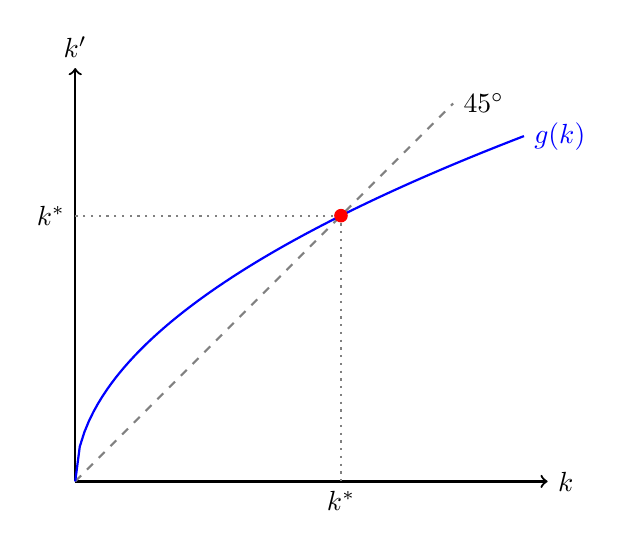
\begin{tikzpicture}[scale=1.5]
    % Axes
    \draw[->, thick] (0,0) -- (4,0) node[right] {$k$};
    \draw[->, thick] (0,0) -- (0,3.5) node[above] {$k'$};
    
    % 45-degree line
    \draw[dashed, thick, gray] (0,0) -- (3.2, 3.2) node[right, text=black] {$45^\circ$};
    
    % Policy function curve g(k) using an exact concave function: k' = 1.5 * sqrt(k)
    \draw[thick, blue, domain=0:3.8, samples=100] plot (\x, {1.5*sqrt(\x)}) node[right] {$g(k)$};
    
    % Helper lines for the steady state
    % Drawing dotted projections to the horizontal and vertical axes
    \draw[dotted, thick, gray] (2.25, 2.25) -- (2.25, 0) node[below, text=black] {$k^*$};
    \draw[dotted, thick, gray] (2.25, 2.25) -- (0, 2.25) node[left, text=black] {$k^*$};
    
    % Intersection point (Steady state) exactly at (2.25, 2.25)
    \filldraw[red] (2.25, 2.25) circle (1.5pt);
\end{tikzpicture}
\end{center}

This phase diagram illustrates the dynamic evolution of capital via the policy function $k' = g(k)$. The horizontal axis represents the current capital stock $k$, and the vertical axis represents tomorrow's capital stock $k'$. The dashed $45^\circ$ line represents the locus of points where $k' = k$ (i.e., capital remains constant). The intersection of the policy function $g(k)$ and the $45^\circ$ line strictly determines the \textit{steady state} of the economy, denoted as $k^*$. Because the policy function $g(k)$ is strictly concave and crosses the $45^\circ$ line from above, the steady state is globally stable: for any initial $k_0 > 0$, the economy will dynamically converge to $k^*$.

\subsection{Solving the Model Numerically: Value Function Iteration}

The mathematical justification for Value Function Iteration relies on functional analysis, specifically the \textit{Banach Fixed-Point Theorem}. Let $T$ be the Bellman operator mapping a value function $V$ into a new value function $TV$:
\[
    (TV)(k) = \max_{k'} \left\{ u(Af(k) + (1-\delta)k - k') + \beta V(k') \right\}
\]
According to \textit{Blackwell's Sufficient Conditions}, because the operator $T$ satisfies \textit{monotonicity} (if $V \ge W$, then $TV \ge TW$) and \textit{discounting} (for any constant $a \ge 0$, $T(V+a) \le TV + \beta a$), the Bellman operator $T$ is a \textbf{contraction mapping} with modulus $\beta \in (0,1)$. 

\thm{Banach Fixed Point Theorem}{
    \begin{itemize}
    \item \textit{Existence and Uniqueness:} There exists a unique true value function $V^*$ such that $TV^* = V^*$ (a unique fixed point).
    \item \textit{Global Convergence:} For \textit{any} initial guess $V^{(0)}$, the sequence generated by $V^{(i+1)} = TV^{(i)}$ will converge to the true value function $V^*$ uniformly as $i \to \infty$. This is the theoretical bedrock that allows us to safely initialize VFI with an arbitrary guess like $V^{(0)}(k) = 0$.
\end{itemize}
}

To solve the recursive Bellman equation computationally, we use an algorithm known as \textit{Value Function Iteration} (VFI). Since a computer cannot process an infinite-dimensional continuous function, we must approach the problem through discretization and recursive iteration.

The standard VFI algorithm proceeds as follows:
\state{Algorithm: Value Function Iteration}{
    \begin{enumerate}
    \item \textbf{Set a grid on the state space:} \\
    Choose a finite set of $n$ discrete grid points for the capital stock: 
    \[ K = \{k_1, k_2, \dots, k_n\} \]

    \item \textbf{Start with an initial guess $V^{(0)}$:} \\
    Initialize the value function for all points on the grid. A common and mathematically valid starting point is zero:
    \[
        V^{(0)}(k) = 0, \quad \forall k \in K
    \]

    \item \textbf{Update the value function using the Bellman Equation:} \\
    For each $k \in K$, compute the updated value function $V^{(i+1)}(k)$ by solving the maximization problem on the right-hand side (RHS). In the most basic version of the algorithm, we restrict the choice variable $k'$ to also be chosen from the discrete grid $K$:
    \[
        V^{(i+1)}(k) = \max_{k' \in K} \left\{ u\underbrace{\left( Af(k) + (1-\delta)k - k' \right)}_{\text{consumption } c} + \beta V^{(i)}(k') \right\}
    \]
    \textit{Note:} The underbrace does not imply $c$ is a constant. It simply indicates that the term inside the parenthesis is the household's consumption level, substituting out the resource constraint.

    \item \textbf{Check for convergence:} \\
    Evaluate the maximum absolute difference (the sup-norm) between the new and old value functions over the entire grid:
    \[
        \max_{k \in K} \left| V^{(i+1)}(k) - V^{(i)}(k) \right| < \epsilon
    \]
    where $\epsilon$ is a pre-specified small tolerance level (e.g., $10^{-6}$).\footnote{\textbf{Coding Practice:} In programming languages like R, Python, or MATLAB, this step is typically implemented using a \texttt{while} loop. To prevent an infinite loop if the algorithm fails to converge (e.g., due to poor calibration or grid issues), you should always code a fail-safe maximum number of iterations: \texttt{while (error > tol) \&\& (iter < max\_iter)}. If the loop terminates because it hits \texttt{max\_iter}, the code should print a warning.}  
    \begin{itemize}
        \item If the condition holds, the value function has converged. Stop the iteration.
        \item Otherwise, set $i \leftarrow i+1$ and return to Step 3.
    \end{itemize}
    
    \item \textbf{Extract the Policy Function} \\
    Once the value function has converged to $V^*$, finding the optimal policy function $k' = g(k)$ requires just one final pass through the state space. For each grid point $k \in K$, we find the $k'$ that maximizes the RHS of the Bellman equation using the converged $V^*$:
    \[
        g(k) = \arg\max_{k' \in K} \left\{ u(Af(k) + (1-\delta)k - k') + \beta V^*(k') \right\}
    \]
    In coding terms, instead of storing the \texttt{max} value as we did during the iteration, we now record the \texttt{argmax} (the optimizer) to recover the optimal path of capital.
\end{enumerate}
}

% Illustration of Discretized Space and VFI Convergence
\begin{center}
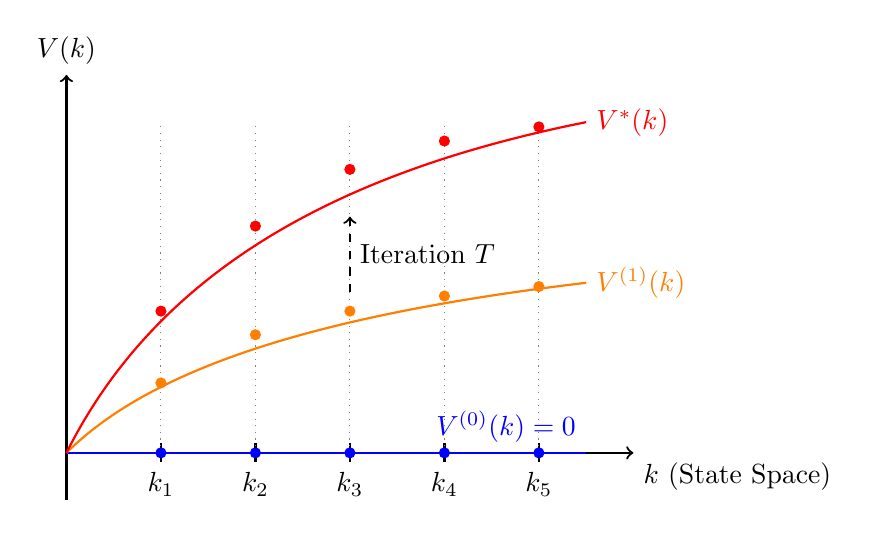
\begin{tikzpicture}[scale=1.2]
    % Axes
    \draw[->, thick] (0,0) -- (6,0) node[below right] {$k$ (State Space)};
    \draw[->, thick] (0,-0.5) -- (0,4) node[above] {$V(k)$};
    
    % Discretized Grid points on x-axis
    \foreach \x in {1, 2, 3, 4, 5} {
        \draw[thick] (\x, 0.1) -- (\x, -0.1) node[below] {$k_\x$};
        \draw[dotted, gray] (\x, 0) -- (\x, 3.5);
    }
    
    % Initial Guess V0 (Adjusted label position to avoid overlap with axis label)
    \draw[thick, blue] (0,0) -- (5.5,0) node[above left] {$V^{(0)}(k) = 0$};
    \foreach \x in {1, 2, 3, 4, 5} \filldraw[blue] (\x, 0) circle (1.5pt);
    
    % V1
    \draw[thick, orange] (0,0) .. controls (1, 1) and (3, 1.5) .. (5.5, 1.8) node[right] {$V^{(1)}(k)$};
    \foreach \x/\y in {1/0.74, 2/1.25, 3/1.5, 4/1.66, 5/1.76} \filldraw[orange] (\x, \y) circle (1.5pt);
    
    % Arrow showing convergence
    \draw[->, thick, dashed] (3, 1.7) -- (3, 2.5) node[midway, right] {Iteration $T$};
    
    % Converged V*
    \draw[thick, red] (0,0) .. controls (1, 2) and (3, 3) .. (5.5, 3.5) node[right] {$V^*(k)$};
    \foreach \x/\y in {1/1.5, 2/2.4, 3/3.0, 4/3.3, 5/3.45} \filldraw[red] (\x, \y) circle (1.5pt);
\end{tikzpicture}
\end{center}

\rmkb[Continuous Choice, Interpolation, and the Curse of Dimensionality]{
In the basic algorithm above, both the current state $k$ and the choice variable $k'$ are restricted to the discrete grid $K$. However, this purely discrete approach creates a fundamental problem: restricting $k'$ to a coarse grid yields highly inaccurate policy functions.

To improve precision without increasing the grid size, advanced numerical solvers allow the choice variable $k'$ to be \textit{continuous}, even though the state space $k$ remains discrete. When a continuous optimizer searches for the optimal $k'$, it will likely select a value that falls \textit{between} two of our pre-defined grid points. Since the computer only stores the value function $V^{(i)}$ at exact grid points, it must guess the value of $V^{(i)}(k')$ using \textbf{interpolation}. Common interpolation methods include:
\begin{itemize}
    \item \textbf{Step function (Nearest-neighbor):} The worst possible method. It rounds $k'$ to the nearest grid point, creating artificial "flat spots" (zero derivatives) and discontinuities. This destroys the strict concavity of the value function, rendering derivative-based First-Order Conditions (FOCs) entirely useless.
    \item \textbf{Piecewise linear interpolation:} Simple and robust, but introduces kinks (non-differentiability) at the grid points.
    \item \textbf{Spline interpolation} (e.g., cubic splines): The ideal method. It preserves the smoothness and strict concavity of the value function, allowing for fast, derivative-based optimization.\footnote{\textbf{Spline Interpolation:} A spline is a mathematical function defined piecewise by polynomials. A \textit{cubic spline} connects the predefined grid points (knots) using third-degree polynomials, matching not just the function values, but also the first and second derivatives at each knot. This ensures the resulting approximated function is globally continuous and smooth.}
\end{itemize}


Then a natural question arises: \textit{Why not simply use a massive discrete grid and avoid interpolation altogether?} \\
Doing so would trigger the \textit{Curse of Dimensionality}. As the number of state variables in a macroeconomic model increases (e.g., adding employment status, idiosyncratic productivity shocks, etc.), the total number of required grid points grows exponentially. For instance, a model with 3 state variables each having 100 grid points requires evaluating $100^3 = 1,000,000$ points per iteration. This exponential explosion in memory usage and computational time forces macroeconomists to keep grid sizes small and rely heavily on continuous choice and sophisticated interpolation methods.
}

\rmkb[Grid Design: Anchoring the Grid Around the Steady State]{
A question that is logically prior to the choice of interpolation method is: \textit{where should the grid points be placed?} The answer is not arbitrary---it depends on both the structure of the model and the specific question being asked.

\medskip
\noindent\textbf{Step 1: Find the steady state first.} Before constructing the grid, it is useful to characterize the steady state $k^*$ at which $g(k^*) = k^*$. Depending on the model, this may be available analytically (e.g., from the Euler equation at steady state) or may itself require a numerical root-finding step. Either way, $k^*$ serves as the natural anchor for grid design.

\medskip
\noindent\textbf{Step 2: Align the grid with the research question.}

\begin{itemize}
    \item \textit{Transition dynamics.} If the goal is to study how an economy converges from a low initial capital stock $k_0 \ll k^*$ toward the steady state---a common question in development economics---then the grid should span $[k_{\min}, k^*]$ (or slightly beyond $k^*$ for symmetry), with points concentrated in the range where the value function and policy function have the most curvature, typically near $k_{\min}$.

    \item \textit{Fluctuations around the steady state.} If instead the goal is to study business-cycle dynamics---small perturbations around $k^*$ induced by productivity shocks---then a narrower grid centered tightly around $k^*$ is more appropriate. Placing many grid points far from $k^*$ wastes computational resources on regions the economy will never visit in the relevant simulation.
\end{itemize}
\rmk{
     A uniformly spaced grid allocates resolution evenly, but the value function and policy function are often much more curved at low $k$ (where the Inada condition implies $f'(k) \to \infty$) and nearly linear near the steady state. A \textbf{log-spaced grid}---evenly spaced in $\log k$ rather than $k$---allocates more points to the low-$k$ region where precision matters most, without requiring an excessively large total number of grid points.
}
}


